\thispagestyle{plain}
\section{Porcentajes}

\boxabstract{Aprendizajes esperados}{Resuelve problemas de cálculo de porcentajes, de tanto por ciento y de la cantidad base.}

\subsection{Tanto por ciento}

\begin{boxK}
    \begin{center}\textbf{Inicio}\end{center}
    \begin{enumerate}
        \item El grupo 1º C ha organizado una competencia para elegir al equipo que los
              representará en el torneo de tiros libres de basquetbol de la escuela. Cada
              equipo está formado por cuatro alumnos y cada uno debe realizar un número distinto
              de lanzamientos a la canasta: uno debe hacer 20, otro 10, otro 5 y
              otro 4. Ganará el equipo que enceste más veces.
              En un equipo están Pablo, Sofía, Alfonso y Nayhelli, quienes en los entrenamientos
              tuvieron el desempeño que muestra la tabla.
              \begin{figure}[H]
                  \centering
                  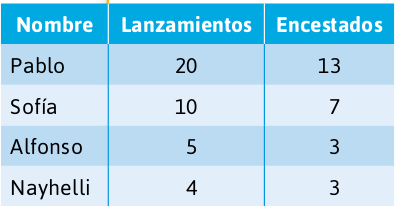
\includegraphics[width=0.4\linewidth]{tabla_lanzamientos.png}
                  \captionof{figure}{}
                  \label{fig:tabla_lanzamientos}
              \end{figure}
              \begin{enumerate}
                  \item ¿Quién es el mejor encestador? ¿Cómo lo sabes?
                  \item ¿Cuántos lanzamientos le asignarías a cada uno para obtener el mejor resultado en la competencia?
                  \item Compara tus respuestas con las de tus compañeros. Respecto a
                        esos cuatro alumnos, ¿cómo decidieron quién es el mejor y el
                        peor encestador? ¿Con qué criterios asignaron el número de
                        lanzamientos a cada uno? Argumenten sus respuestas.
              \end{enumerate}

    \end{enumerate}
\end{boxK}

\begin{enumerate}
    \item En la Academia de Policía evaluaron la condición física de los cadetes.
          \begin{enumerate}
              \item Marca las afirmaciones equivalentes.\\
                    \begin{hoptboxes}
                        \item Tres quintas partes tuvo excelentes resultados.\\
                        \item Veinte de cada veinticinco cadetes tuvieron excelentes resultados.\\
                        \item De cada cinco alumnos, cuatro lograron excelentes resultados.\\
                        \item De cien cadetes, ochenta tuvieron excelentes resultados.\\
                        \item Ocho de cada diez lograron excelentes resultados.\\
                    \end{hoptboxes}
              \item Compara tus respuestas con las de tus compañeros y explíquenlas.
              \item Expresa en cada caso el número de cadetes con buenos resultados como una fracción
                    con denominador 100. ¿Qué observas?
          \end{enumerate}

          \begin{boxH}
              Por ciento significa \emph{por cada cien} y se refiere a la razón entre una cantidad dada
              y un total de 100 elementos; también se llama tanto por ciento, esto es, \emph{una cantidad por cada cien}.
              Se usa el símbolo \% para indicar un tanto por ciento: 27 de
              cada 100 se expresa como 27 o 27\%.
          \end{boxH}

    \item Completa la tabla \ref{fig:tabla_tantoporciento}.

          \begin{figure}[H]
              \centering
              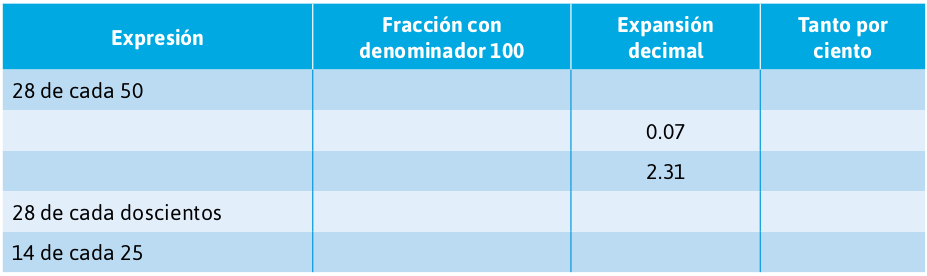
\includegraphics[width=0.7\linewidth]{tabla_tantoporciento.png}
              \captionof{figure}{}
              \label{fig:tabla_tantoporciento}
          \end{figure}

          \begin{enumerate}
              \item En su cuaderno escriban qué relación hay entre la expansión decimal y el tanto por
                    ciento.
          \end{enumerate}
    \item Escribe el tanto por ciento que representa la parte sombreada de las
          figuras o coloreen el porcentaje que corresponde.
          \begin{figure}[H]
              \centering
              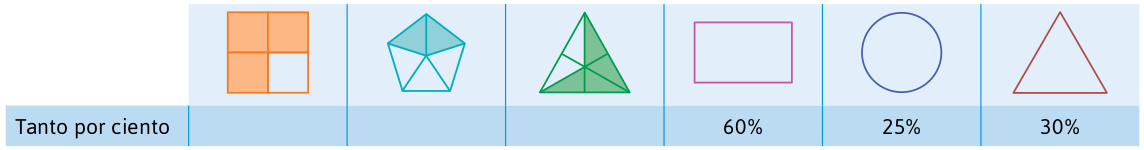
\includegraphics[width=0.8\linewidth]{tabla_figuras.png}
              \captionof{figure}{}
              \label{fig:tabla_figuras}
          \end{figure}
          \begin{boxH}
              Para convertir un decimal en tanto por ciento, se multiplica el decimal por 100 y
              se agrega el signo \%.
          \end{boxH}
\end{enumerate}

\begin{boxK}
    \begin{center}\textbf{Cierre}\end{center}

    \begin{enumerate}
        \item Retoma la actividad de la situación inicial y determina el porcentaje de encestes
              con respecto a los lanzamientos de cada alumno.
              \begin{enumerate}
                  \item Resuelve nuevamente el inciso b. Explica cómo llegaste a esa conclusión.
                  \item ¿Tus resultados iniciales fueron correctos? Justifica tus respuestas.
              \end{enumerate}
        \item El promedio de bateo se determina como la razón del número de hits que logra
              un jugador de beisbol entre la cantidad de turnos al bat.\\
              \begin{enumerate}
                  \item  El legendario jugador de beisbol Babe Ruth de los Yanquis de Nueva York tuvo
                        un promedio de bateo de 0.34. ¿Qué significa ese número en porcentaje?
                  \item Adrián \emph{el titán} González, bateador mexicano de los Dodgers de Los Ángeles,
                        tiene promedio de bateo de 0.29. ¿Quién es mejor bateador? Explica.
              \end{enumerate}
    \end{enumerate}
\end{boxK}
\newpage
\subsection{Cálculo del porcentaje}

\begin{boxK}
    \begin{center}\textbf{Inicio}\end{center}

    \begin{enumerate}
        \item Observa los anuncios.
              \begin{figure}[H]
                  \centering
                  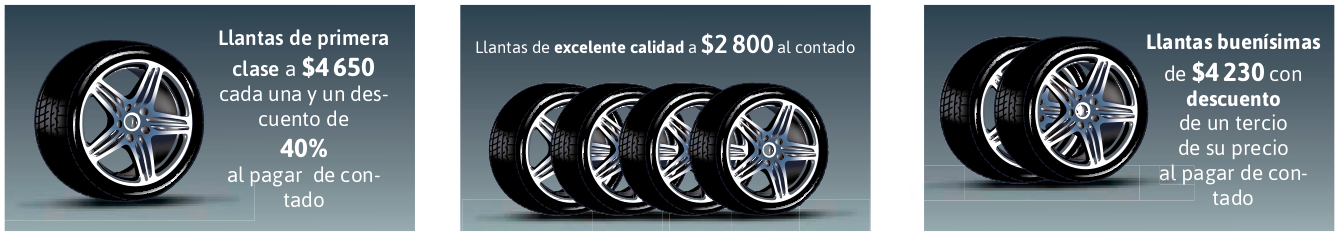
\includegraphics[width=\linewidth]{llantas.png}
                  % \captionof{figure}{}
                  % \label{fig:llantas}
              \end{figure}
              \begin{enumerate}
                  \item Cuál es la mejor oferta si todas las llantas son del mismo tipo y marca?
                  \item Compara tu respuesta con la de tus compañeros y argumenten por qué su elección es la mejor.
              \end{enumerate}
    \end{enumerate}
\end{boxK}
\begin{enumerate}
    \item Observa la nota del consumo del restaurante de la figura \ref{fig:nota_consumo} y
          contesten.

          \begin{minipage}[t]{0.2\textwidth}
              \begin{figure}[H]
                  \centering
                  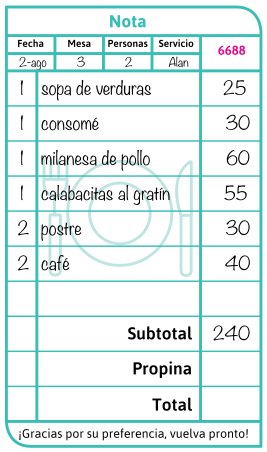
\includegraphics[width=\linewidth]{nota_consumo.png}
                  \captionof{figure}{}
                  \label{fig:nota_consumo}
              \end{figure}
          \end{minipage}\hfill
          \begin{minipage}[t]{0.75\textwidth}
              \begin{enumerate}
                  \item Como propina, los comensales quieren dejar 10\% del precio de su consumo. ¿Qué cantidad deben anotar en la nota?\\
                  \item Y si la cuenta fuera de \$534.00, ¿cuánto sería de propina?\\
                  \item Escriban un procedimiento para obtener el 10\% de una cantidad.\\
                  \item Comparen sus procedimientos con los del grupo. ¿Son iguales o diferentes? ¿Todos son correctos? Argumenten sus respuestas y valídenlas en grupo.\\
              \end{enumerate}
          \end{minipage}

          \begin{boxH}
              Cuando a una cantidad se aplica el tanto por ciento se involucran tres
              datos: el tanto por ciento o \textbf{tasa}, la cantidad a la que se le aplica esa tasa
              (\textbf{cantidad base}) y el resultado (\textbf{porcentaje}).
          \end{boxH}
    \item Calcula los porcentajes.
          \begin{enumerate}
              \item Obten el 10\% de las siguientes cantidades.\\

                    \begin{hoptions}
                        \item 25 \rule{20mm}{0.2mm}
                        \item 36.8 \rule{20mm}{0.2mm}
                        \item 2445.9 \rule{20mm}{0.2mm}
                        \item 66 \rule{20mm}{0.2mm}
                    \end{hoptions}
              \item Obten el 5\%.\\

                    \begin{hoptions}
                        \item 25 \rule{20mm}{0.2mm}
                        \item 36.8 \rule{20mm}{0.2mm}
                        \item 2445.9 \rule{20mm}{0.2mm}
                        \item 66 \rule{20mm}{0.2mm}
                    \end{hoptions}
              \item Calcula el 20\%.\\

                    \begin{hoptions}
                        \item 25 \rule{20mm}{0.2mm}
                        \item 36.8 \rule{20mm}{0.2mm}
                        \item 2445.9 \rule{20mm}{0.2mm}
                        \item 66 \rule{20mm}{0.2mm}
                    \end{hoptions}
              \item ¿Qué procedimiento seguiste para obtener los resultados? Explícalo al resto del grupo y valídenlos.\\
              \item Explica cómo calcular mentalmente el 1\% de cualquier cantidad.\\
          \end{enumerate}
    \item Calcula el 1\% de las siguientes cantidades.\\

          \begin{hoptions}
              \item 115.1 \rule{20mm}{0.2mm}
              \item 780 \rule{20mm}{0.2mm}
              \item 300 \rule{20mm}{0.2mm}
              \item 66.6 \rule{20mm}{0.2mm}
          \end{hoptions}
    \item Calcula los porcentajes de las cantidades de la tabla \ref{fig:tabla_porciento}.\\

          \begin{figure}[H]
              \centering
              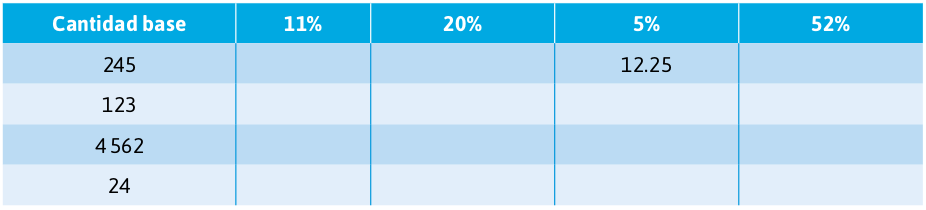
\includegraphics[width=.8\linewidth]{tabla_porciento.png}
              \captionof{figure}{}
              \label{fig:tabla_porciento}
          \end{figure}
    \item Realiza los siguientes ejercicios.
          \begin{enumerate}
              \item Calculen el 35\% de 240 pesos.
              \item Escriban 35\% como una fracción con denominador 100.
              \item Completen la siguiente proporción.
                    \[\dfrac{35}{100} = \dfrac{}{240}\]
              \item Comparen su resultado con el inciso a. ¿Qué observan?
              \item Expliquen cómo calcular el porcentaje de una cantidad dada la tasa. Compartan
                    sus propuestas en grupo y propongan ejercicios para aplicarlas. Verifiquen los
                    resultados y utilícenlos como validación de sus procedimientos.
          \end{enumerate}
    \item Analiza la afirmación del recuadro.
          \begin{boxH}
              Para calcular el porcentaje de una cantidad basta multiplicar la cantidad base por
              la tasa y dividir entre 100.
          \end{boxH}
          \begin{enumerate}
              \item ¿Es correcta? ¿Por qué?
          \end{enumerate}
\end{enumerate}

\begin{boxK}
    \begin{center}\textbf{Cierre}\end{center}

    \begin{enumerate}
        \item Retoma la actividad de la situación inicial y según lo que aprendiste en la lección
              determina cuál es la oferta más económica. Observa que el hecho de
              anunciar un gran descuento no significa forzosamente un precio más barato.
        \item En una tienda anuncian un 20\% de descuento en todos sus productos. Observa
              la computadora.
              \begin{enumerate}
                  \item ¿Cuál es su precio después de la rebaja? ¿Cómo obtuviste ese resultado?
                  \item Calcula el 80\% del precio de la computadora y compara tu resultado con el del inciso a. ¿Qué observas?
                  \item ¿Cómo calcularías el precio con descuento de una televisión que cuesta \$2 340.00? Indica su precio final.
                  \item Compara tus resultados y procedimientos con los de tus compañeros y valídenlos con ayuda de su profesor.
              \end{enumerate}
    \end{enumerate}
\end{boxK}
\newpage
\subsection{Porcentajes y aplicaciones}
\begin{boxK}
    \begin{center}\textbf{Inicio}\end{center}

    \begin{enumerate}
        \item El entrenador de un equipo de beisbol debe comprar guantes y bates para todo el equipo.
              Revisa las ofertas de las tiendas El guante de oro y El bateador.
              \begin{figure}[H]
                  \centering
                  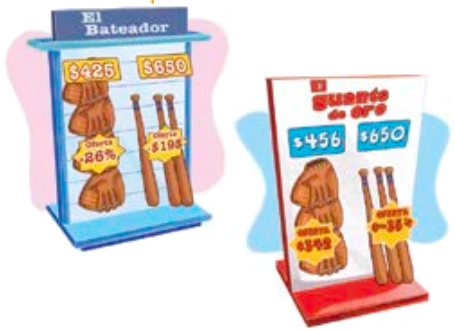
\includegraphics[width=.5\linewidth]{tiendas.png}
                  \captionof{figure}{}
                  \label{fig:tiendas}
              \end{figure}
              \begin{enumerate}
                  \item ¿En qué tienda el guante tiene mayor descuento en pesos?
                  \item ¿En cuál tiene mayor tasa de descuento?
                  \item ¿En cuál tienda son más baratos los bates?
                  \item ¿Cuáles bates tienen mayor tasa de descuento?
                  \item ¿Dónde comprarías tres bates y nueve guantes?
                  \item ¿Cuánto pagarías y cuánto ahorrarías?
                  \item Compara tus resultados y tus procedimientos con los de tus
                        compañeros y argumenten por qué piensan que su elección
                        es correcta.
              \end{enumerate}
    \end{enumerate}
\end{boxK}

\begin{enumerate}
    \item La gráfica muestra la composición de una escuela de 2 400 personas.
          \begin{figure}[H]
              \centering
              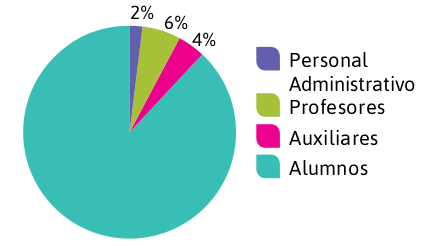
\includegraphics[width=.5\linewidth]{escuela_pie.png}
              \captionof{figure}{}
              \label{fig:escuela_pie}
          \end{figure}
          \begin{enumerate}
              \item ¿Cuántas personas trabajan en la administración?
              \item ¿Cuántos profesores hay en esa escuela?
              \item ¿Cuántas personas son auxiliares?
              \item ¿Cuál es el porcentaje de alumnos?
              \item ¿Cuántos alumnos tiene la escuela?
          \end{enumerate}
    \item Don Lupe es carpintero y comenta que el precio de la madera aumentó 8\%, por lo
          que piensa cobrar 8\% más en todos los muebles y objetos que fabrique.
          \begin{figure}[H]
              \centering
              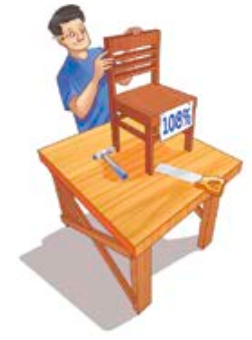
\includegraphics[width=.3\linewidth]{donLupe.png}
              \captionof{figure}{}
              \label{fig:donLupe}
          \end{figure}
          \begin{enumerate}
              \item Él considera que cobrando el 108\% del precio original de sus productos
                    estaría cobrando el incremento que pretende. ¿Su razonamiento es correcto? Explica.
              \item ¿Cuál sería el nuevo precio de una silla que costaba \$250 pesos?
          \end{enumerate}
    \item En una tienda departamental Constanza compró el juego de sartenes que muestra
          el anuncio. El precio original era de \$348.00 y la cajera le comentó que sobre el
          precio final debía pagar el 16\% de IVA. Constanza sugirió pagar primero el IVA y
          después aplicar el descuento para, de esa manera, pagar menos.
          \begin{figure}[H]
              \centering
              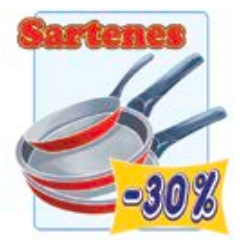
\includegraphics[width=.3\linewidth]{sartenes.png}
              \captionof{figure}{}
              \label{fig:sartenes}
          \end{figure}
          \begin{enumerate}
              \item ¿El razonamiento de Constanza es correcto? Explica.
              \item Compartan sus respuestas en grupo. ¿Creen que es mejor primero cobrar el IVA y
                    luego hacer el descuento o al revés? ¿Por qué?
          \end{enumerate}
    \item Resuelve los siguientes problemas.
          \begin{enumerate}
              \item En la papelería La goma todos los precios incluyen IVA. Si el impuesto
                    (16\%) que se paga por los colores es de \$4.00, ¿cuál es su precio sin IVA?
              \item En la misma papelería el papel para dibujo está en oferta. Si al precio,
                    \$165.00, se le descuentan \$24.75, ¿de cuánto es la tasa de descuento?

              \item ¿Cómo obtuvieron el resultado de cada uno de los incisos anteriores? Expliquen
                    sus procedimientos ante el grupo y entre todos propongan procedimientos para
                    calcular la cantidad base dadas la tasa y el porcentaje, y para obtener la tasa,
                    dadas la cantidad base y el porcentaje.
          \end{enumerate}
\end{enumerate}

\begin{boxK}
    \begin{center}\textbf{Cierre}\end{center}

    Retoma la actividad de la situación inicial y determina dónde es más conveniente
    comprar cada artículo deportivo. ¿Cuánto se ahorraría? ¿Coinciden tus
    respuestas con las que obtuviste al inicio? Valídalas con el resto del grupo
\end{boxK}

\begin{boxH}
    Como en la mercería \emph{El resguardo} están reetiquetando toda la mercancía, el gerente
    indica que el precio en la etiqueta debe incluir un descuento de 5\% y el 16\%
    del IVA . Una empleada piensa que basta con aumentar los precios un 11\%. ¿Su razonamiento
    es correcto? Justifica tu respuesta con ejemplos.
\end{boxH}



\newpage